\documentclass[12pt,a4paper]{article}
\usepackage{algorithm, algpseudocode, amsmath, amssymb, amsthm, bm, csquotes, emf, empheq, geometry, graphicx, hyperref, listings, mhchem, multirow, siunitx, slashbox, subcaption, upgreek}
\usepackage[italicdiff]{physics}
%\usepackage[section]{placeins}
\usepackage[justification=centering]{caption}
\usepackage[column=O]{cellspace}
\usepackage[extrafootnotefeatures]{xepersian}
\hypersetup{colorlinks=true, urlcolor=cyan}

\title{نورسنجی خوشه}
\author{آرتین خانعلی، سپهر سلمانی یگانه، صالح شاملو احمدی\\\\
	آزمایشگاه نجوم، ترم تابستان ۱۴۰۲\\دانشکده فیزیک دانشگاه صنعتی شریف}
\date{۱۳ شهریور ۱۴۰۲}

\settextfont{Yas}
%\ExplSyntaxOn
%\cs_set_eq:NN
%\etex_iffontchar:D
%\tex_iffontchar:D
%\cs_undefine:N \c_one
%\int_const:Nn \c_one { 1 } 
%\ExplSyntaxOff
%\setdigitfont{Yas}
\linespread{1.2}

\makeatletter
\g@addto@macro\bfseries{\boldmath}
\makeatother

\setlength\cellspacetoplimit{5pt}
\setlength\cellspacebottomlimit{3pt}
\newcommand{\multlinecell}[1]{\begin{tabular}[c]{@{}c@{}}#1\end{tabular}}

\newcommand{\qfrac}[2]{\left(\frac{#1}{#2}\right)}
\newcommand{\fsqrt}[2]{\sqrt{\frac{#1}{#2}}}
\newcommand{\ddfrac}[2]{{\displaystyle\frac{\displaystyle #1}{\displaystyle #2}}}
\newcommand{\pdvc}[3]{\qfrac{\partial #1}{\partial #2}_{#3}}
\newcommand{\dbar}{{d\mkern-7mu\mathchar'26\mkern-2mu}}
\newcommand*{\defeq}{\mathrel{\vcenter{\baselineskip0.5ex \lineskiplimit0pt
			\hbox{\scriptsize.}\hbox{\scriptsize.}}}
	=}

\newtheorem{theorem}{قضیه}
\newtheorem{lemma}{لم}
\renewcommand\qedsymbol{$\blacksquare$}

\begin{document}
	\maketitle
	%\twocolumnfootnotes
	\section{مقدمه}
	در این آزمایش با هم‌خط کردن عکس‌های متعدد و انجام اصلاحات، یک عکس نجومی مناسب بدست می‌آوریم و
	با استفاده از آن ستاره‌های داخل یک خوشه را نورسنجی می‌کنیم.
	\section{روش آزمایش}
	ابزار مورد استفاده ما در این آزمایش عبارت‌اند از:
	\begin{itemize}
		\item تلسکوپ نیوتنی هشت اینچی (بدون فیلتر)
		\item دوربین \lr{Canon EOS 1200D}
		\item مقر و موتور
	\end{itemize}
	محل رصد، روستای ازناوه واقع در نزدیکی شهر کاشان است. عکس‌ها با نوردهی $1.6$ ثانیه و \lr{ISO $1600$}
	در ساعت ۳۰:۱ تا ۲:۱۸ بامداد ۲۸ تیر ۱۴۰۲ گرفته شده‌اند. عکس‌هایی با نوردهی $1.6$ هم گرفته شده بود
	که به دلیل رَد داشتن قابل استفاده نیستند. پس از قطبی کردن و اطمینان از نوردهی، از خوشه دوتایی
	(خوشه‌های $\chi Persei$ و $h Persei$) با فاصله زمانی یک تا سه دقیقه عکس‌برداری کردیم. پس از رصد،
	در سپیده‌دم با عکس‌برداری بیرون از فکوس از آسمان، فریم‌های \lr{flat} را با نوردهی $2.5$ ثانیه و \lr{ISO $1600$}
	گرفتیم و در آخر با بستن دریچه دوربین و عکس‌برداری در نوردهی و \lr{ISO}های مربوطه، فریم تاریک و
	فریم تاریک \lr{flat} را گرفتیم. برای محاسبه ارتفاع ستاره‌ها در آسمان، از نرم افزار \lr{Starry Night} استفاده کردیم.
	\section{اصلاح عکس‌ها}
	برای کم کردن جریان تاریک عکس، فریم تاریک با نوردهی مناسب (و میانه‌گرفته شده) را از عکس کم کردیم.
	سپس با تقسیم مقادیر پیکسل‌های عکس \lr{flat} بر میانه آن‌ها، \lr{gain table} را ساختیم و مقادیر پیکسل‌های
	عکس را بر مقادیر آن تقسیم کردیم تا عدم نوردهی یکنواخت پیکسل‌ها برطرف شود.
	
	سپس با مقایسه فریم تاریک با دو نوردهی متفاوت، پیکسل‌های مرده را پیدا کردیم که از تحلیل نهایی حذف شده‌اند.
	برای پیدا کردن پیکسل‌های مرده، ابتدا پیکسل‌های «داغ» را پیدا می‌کنیم (پیکسل‌هایی که مقدار بیش از حد بالایی دارند).
	سپس نمودار مقدار ای پیکسل‌ها در دو نوردهی برحسب هم را رسم می‌کنیم. اگر پیکسل‌ها مرده نباشند، باید روی یک خط
	گذرنده از مبدأ قرار بگیرند. این بدان معنی است که مقدار این پیکسل‌ها برحسب نوردهی قابل پیشبینی است که یعنی
	پاسخ نوری پیکسل‌ها سالم است. به دلیل وجود داده‌های پرت، نمی‌توانیم به پیکسل‌ها خط فیت کنیم، و از طرفی به دلیل
	وجود بایاس، شیب خط دقیقاً برابر با نسبت نوردهی‌ها نیست. بنابراین مجبوریم با سعی و خطا شیب خط را پیدا کنیم که
	زیاد سخت نیست. پس از رسم خط، پیکسل‌هایی که بیش از ۲۰ درصد با این خط فاصله دارند را به عنوان پیکسل مرده در نظر
	می‌گیریم. دقت کنید که پیکسل‌هایی که مقدار به نسبت کمتری دارند (از بقیه به وضوح جدا هستند) شامل این قاعده نمی‌شوند
	و آن‌ها را با یک مرز جدا می‌کنیم.
	
	در آخر، برای تحلیل داده ساده‌تر، با نسبت‌های مناسب سه کانال رنگی را ترکیب کردیم تا تصویر سیاه و سفید شود.
	با توجه به اینکه فضای رنگی عکس‌های استفاده شده، \lr{sRGB} است، روشنایی نسبی برحسب سه کانال رنگی برابر است با
	\begin{equation}
		\text{\lr{grayscale intensity}} = 0.2126r + 0.7152g + 0.0722b.
	\end{equation}
	این اعداد مربوط به حساسیت چشم انسان است (چشم به رنگ سبز حساس‌تر است).
	\begin{figure}
		\centering
		\begin{subfigure}{0.49\linewidth}
			\centering
			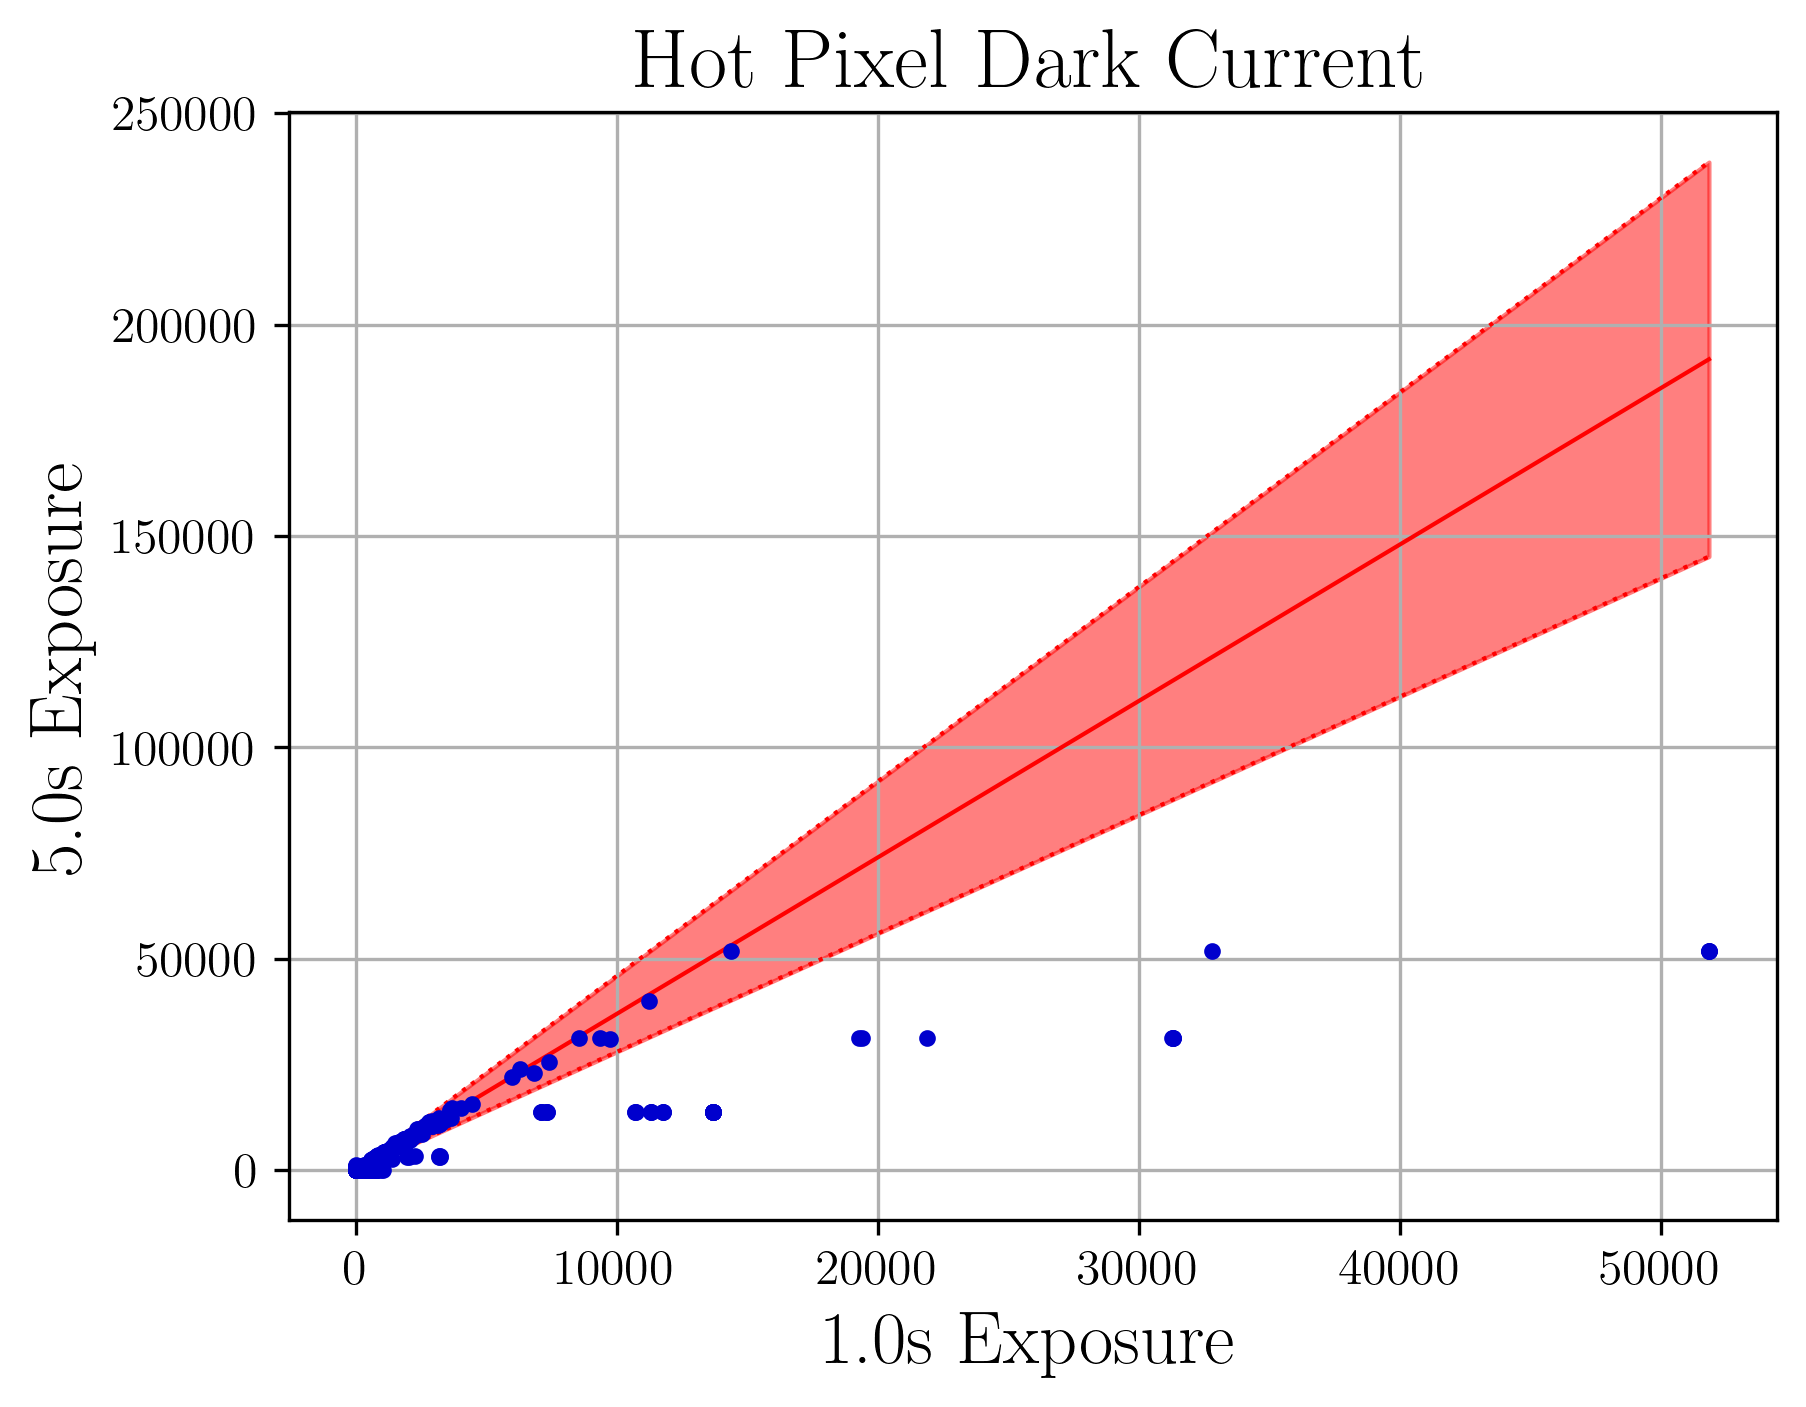
\includegraphics[width=\linewidth]{../fig/hotpix}
		\end{subfigure}
		\begin{subfigure}{0.49\linewidth}
			\centering
			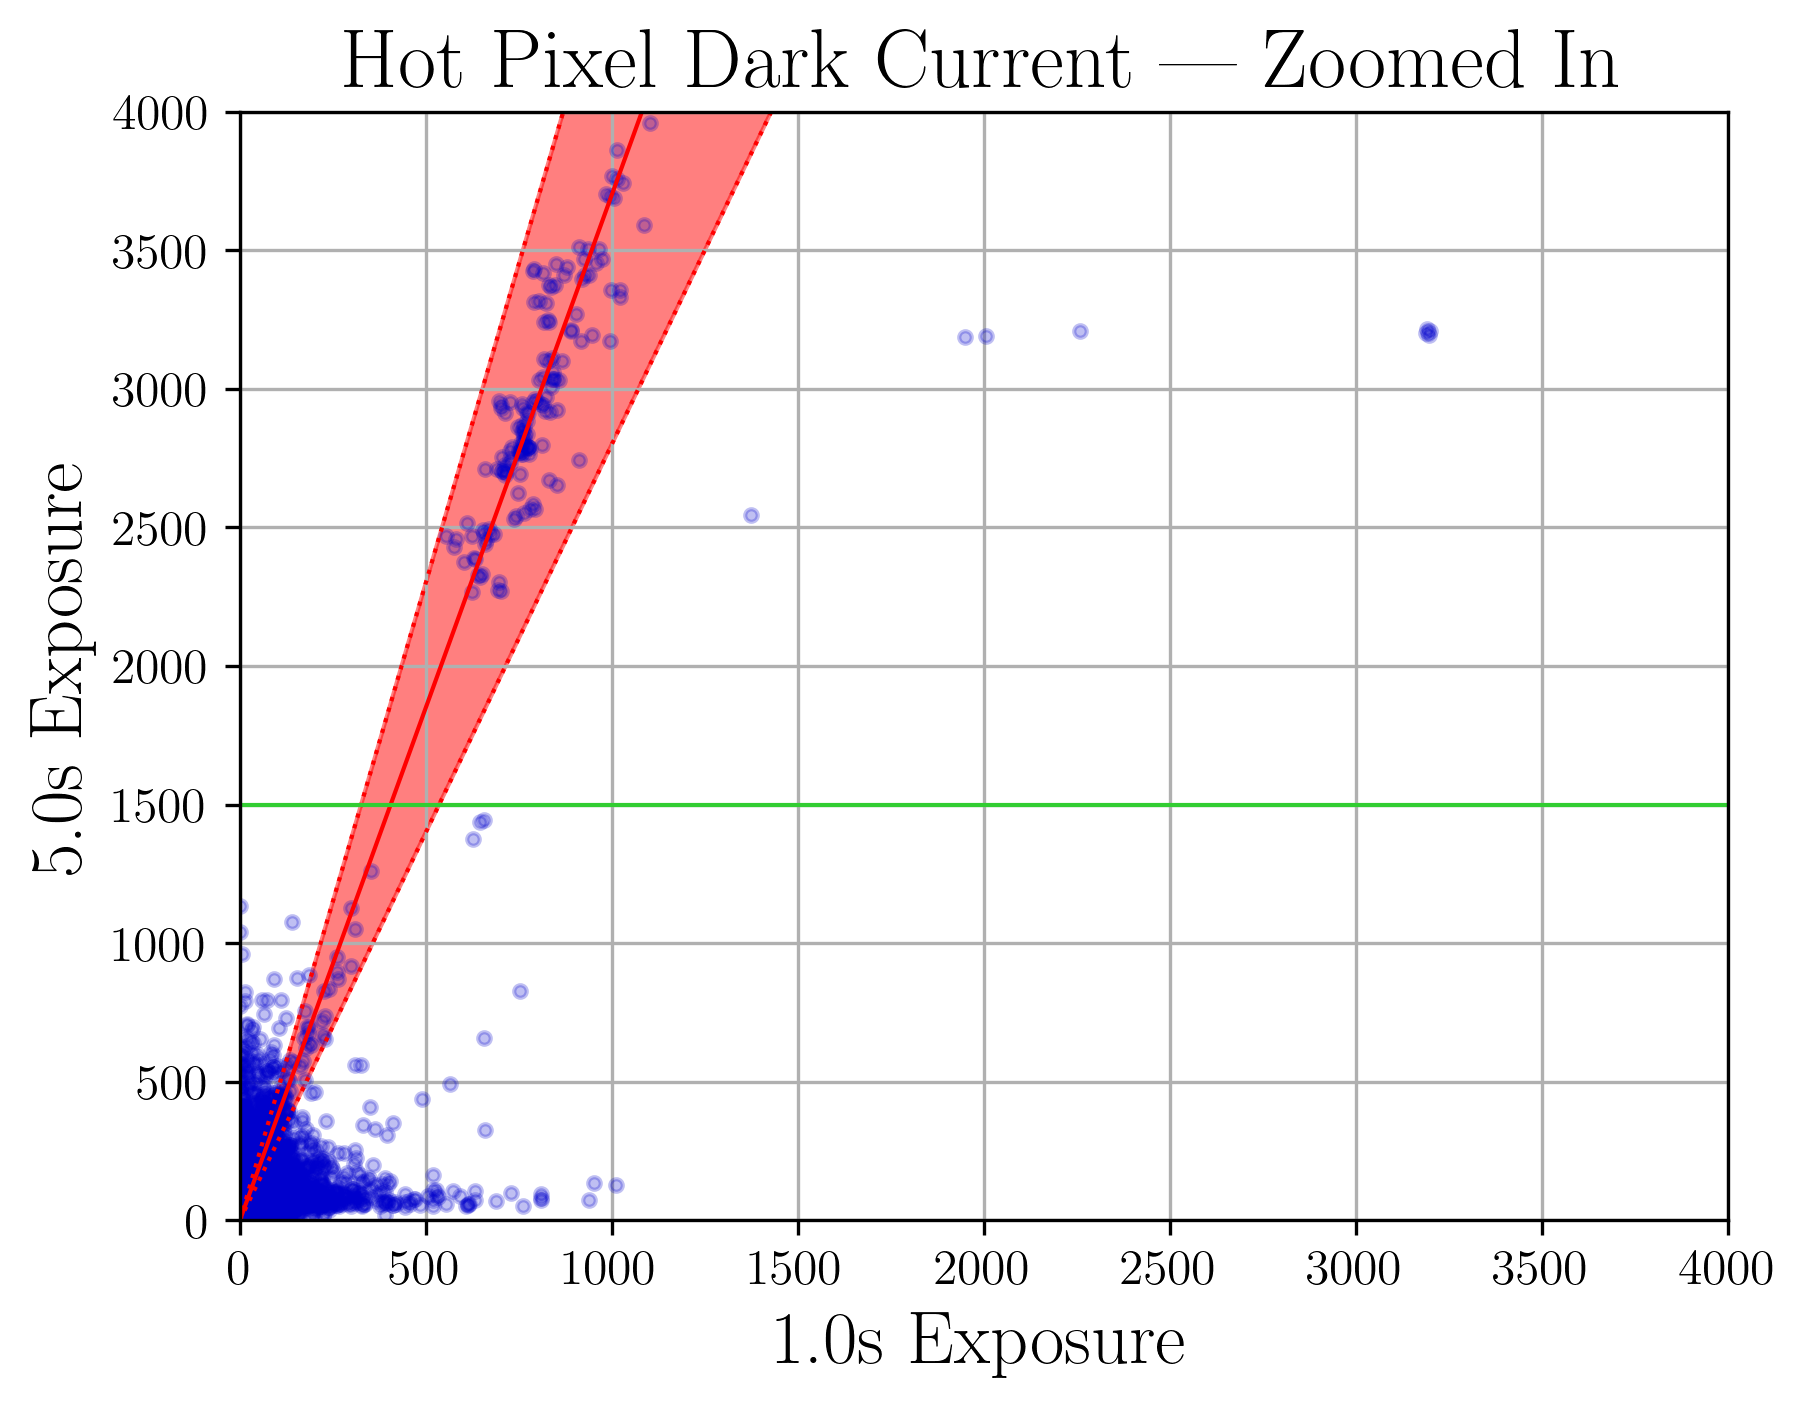
\includegraphics[width=\linewidth]{../fig/hotpix_zoom}
		\end{subfigure}
		\caption{نمودار پیکسل‌های داغ. پیکسل‌های خارج محدوده رنگی حذف می‌شوند.}
	\end{figure}
	\section{هم‌خط کردن عکس‌ها}
	برای بهتر شدن وضوح تصویر نهایی، تصاویر را هم‌خط\footnote{\lr{align}} می‌کنیم. برای این منظور، از پکیج \lr{\texttt{astroalign}}
	استفاده کردیم. این پکیج ابتدا ستاره‌ها را در دو تصویر پیدا می‌کند، سپس بین هر سه‌تا از آن‌ها مثلث می‌کشد
	و سعی می‌کند تبدیلی پیدا کند که یک تصویر را طوری به تصویر دیگر ببرد که این مثلث‌ها روی هم بیفتند.
	بعد از انداختن عکس‌ها روی هم توسط \lr{\texttt{astroalign}}، تصاویر را جمع زدیم و بخش مشترک در تمام تصاویر را بریدیم
	و به صورت فایل \lr{\texttt{FITS}} با عمق ۳۲ بیت ذخیره کردیم (تا از اشباع شدن ستاره‌ها جلوگیری کنیم). برای عکس نهایی،
	بیست عکس مناسب را هم‌خط کردیم.
	
	روش‌های دیگری برای هم‌خط‌سازی براساس قدر ستاره‌ها وجود دارد، اما این روش‌ها دقت کمتری دارند. همچنین نرم‌افزار
	سیریل\footnote{\lr{Siril}} روش‌های متنوع‌تری دارد، اما ترجیح ما بر این بود که تمام مراحل داخل کُد پایتون انجام شود.
	\section{نورسنجی}
	برای نورسنجی \lr{PSF} از پکیج \lr{\texttt{photutils}} استفاده کردیم. برای نورسنجی، ابتدا با روش \lr{DAOFIND} مکان
	اولیه ستاره‌ها پیدا می‌شود.
	
	\lr{DAOFIND} ابتدا با یک کرنل گوسی (با اندازه از پیش تعیین شده) تصویر را تار می‌کند
	(با \lr{convolution}) و سپس پیک‌های تصویر (که بزرگ‌تر از یک حد خاص هستند) را به عنوان ستاره در نظر می‌گیرد. کمینه
	پیک‌ها را میانه به اضافه سه برابر انحراف معیار تصویر در نظر گرفتیم.
	
	بعد از \lr{DAOFIND} و یک تخمین اولیه از شار ستاره‌ها با نورسنجی با دهانه کوچک، تابع گوسی
	در باکس هفت پیکسل در هفت پیکسل به هسته ستاره‌ها فیت می‌شود و انتگرال این تابع به عنوان
	شار ستاره در نظر گرفته می‌شود.
	\section{نتایج}
	در جدول قدر ده ستاره پرنور تصویر آورده شده. این ستاره‌ها در شکل \ref{fig:cluster} شماره‌گذاری شده‌اند. ستاره مرجع
	برای تعیین قدر، ستاره $9$ (\lr{FZ Persei}) است. بقیه داده‌ها در فایل \lr{\texttt{psfphotometry.csv}} واقع در فولدر
	\lr{\texttt{data}} قابل مشاهده‌اند.
	\begin{figure}
		\centering
		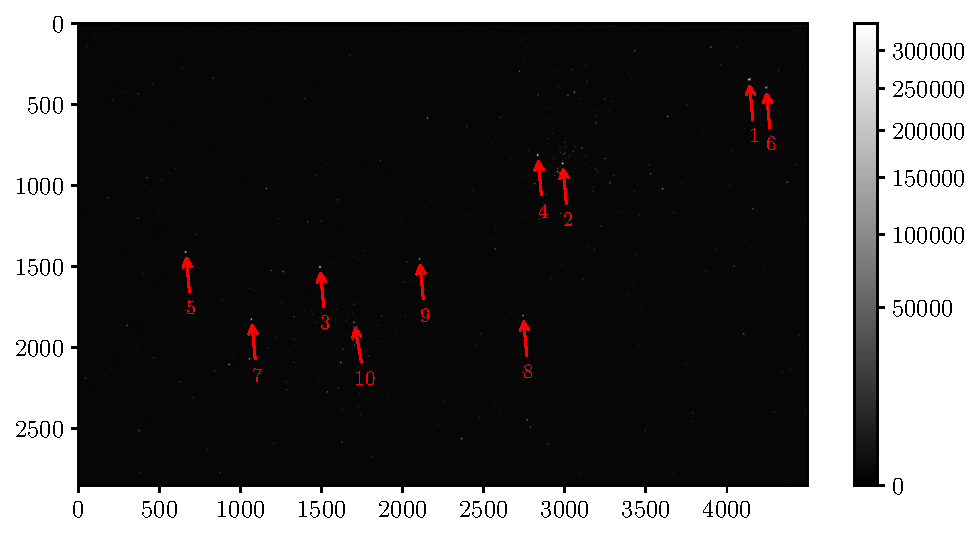
\includegraphics[width=\linewidth]{../fig/cluster}
		\caption{تصویر نهایی خوشه دوتایی با شماره‌گذاری ستاره‌ها. برای بهتر دیده شدن ستاره‌ها، 
				مقادیر پیکسل‌ها به صورت رادیکالی بهنجار شده‌اند.}
		\label{fig:cluster}
	\end{figure}
	\begin{table}
		\centering
		\caption{قدرهای ده ستاره پرنور تصویر.}
		\begin{tabular}{|c|c|c|c|c|}
			\hline
			شماره & $x$ مرکز & $y$ مرکز & قدر مشاهده‌ای & خطای قدر \\ \hline
			$1$ & $4137.36$ & $347.33$ & $6.29$ & $0.08$ \\ \hline
			$2$ & $2987.3$ & $864.48$ & $6.6$ & $0.07$ \\ \hline
			$3$ & $1490.8$ & $1502.59$ & $6.77$ & $0.06$ \\ \hline
			$4$ & $2833.56$ & $812.57$ & $6.79$ & $0.07$ \\ \hline
			$5$ & $662.64$ & $1410.26$ & $7.02$ & $0.05$ \\ \hline
			$6$ & $4241.78$ & $397.25$ & $7.39$ & $0.04$ \\ \hline
			$7$ & $1068.13$ & $1824.24$ & $7.51$ & $0.04$ \\ \hline
			$8$ & $2743.28$ & $1802.19$ & $7.85$ & $0.04$ \\ \hline
			$9$ & $2104.94$ & $1453.79$ & $7.96$ & $0.02$ \\ \hline
			$10$ & $1700.86$ & $1843.72$ & $8.07$ & $0.04$ \\ \hline
		\end{tabular}
	\end{table}
\end{document}